\chapter{Parking Lot}
\label{ch:lot}

\section{Accelerator / Sytem Integration}

The degree to which these accelerators are integrated with the host system varies.
Figure~\ref{fig:integration-spectrum} depicts how integrated some common accelerators are.
Fully-integrated accelerators are characterized by direct and transparent access to system memory, no additional programming system or compiler support, and no explicit control through an OS or vendor API.
For example, floating-point accelerators are fully integrated.
They have migrated into the host instruction-set architecture, have first-class access to system memory, and are supported without specialized toolchains or programming systems.
Similarly, SIMD vector extensions are nearly as integrated, but may require some special attention to memory alignment, precision, or rounding modes.
In contrast, fully-discrete accelerators have their own memory, have esoteric programming systems, and demand explicit control.
For example, FPGAs are programmed in hardware-description languages, may require the host system to be rebooted to be reconfigured, and often require the programmer to explicity transfer data to their memory.
As on the of the most mature accelerators, GPUs occupy a middle ground.
GPUs vary from partially-integrated to discrete: when a GPU is integrated on the same die as the CPU, it may share the same physical memory, but the computation model remains for compute tasks to be ``offloaded'' to the GPU, with the CPU managing the execution.

\begin{figure}
    \centering
    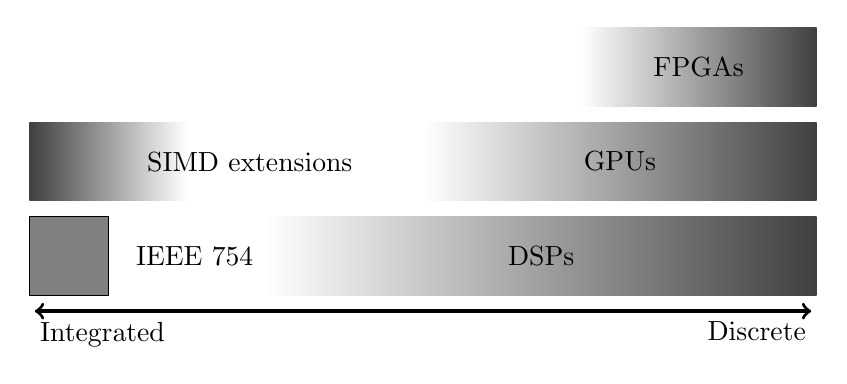
\begin{tikzpicture}[
        nodestyle/.style={},
        axisline/.style={
            <->,
            very thick,
            shorten <=2pt,
            shorten >=2pt,},
        axistext/.style={},
        ]

        \pgfmathsetmacro{\rt}{1} % thickness
        \pgfmathsetmacro{\rs}{0.2} % spacing

        \pgfmathsetmacro\ra{\rs}
        \pgfmathsetmacro\rb{\ra+\rt+\rs}
        \pgfmathsetmacro\rc{\rb+\rt+\rs}


        \draw[axisline] (0,0) node[anchor=north west] {Integrated} -- (10,0) node[anchor=north east] {Discrete};

        \draw[fill=gray] (0,\ra) rectangle (1,\ra+\rt);
        \node [above] at (2.1, \ra+0.25\rt) {IEEE 754};

        \shade[left color=darkgray, right color=white] (0,\rb) rectangle (2,\rb+\rt);
        \node [above] at (2.8, \rb+0.25\rt) {SIMD extensions};

        \shade[left color=white, right color=darkgray] (3,\ra) rectangle (10,\ra+\rt) node[pos=0.5] {DSPs};
        \shade[left color=white, right color=darkgray] (5,\rb) rectangle (10,\rb+\rt) node[pos=0.5] {GPUs};
        \shade[left color=white, right color=darkgray] (7,\rc) rectangle (10,\rc+\rt) node[pos=0.5] {FPGAs};

    \end{tikzpicture}
    \caption{Spectrum of integration for accelerators.}
    \label{fig:integration-spectrum}
\end{figure}


\section{Extensions}
\subsection{cudaMemAdviseSetReadMostly}
\begin{itemize}
    \item CPU-GPU coherence bandwidth (r/w, x access patterns)
    \item GPU-GPU coherence bandwidth (r/w, x access patterns)
    \item estimate invalidation cost (CPU-GPU, GPU->GPU)
\end{itemize}

\subsection{System Atomics}
\begin{itemize}
    \item Latency and throughput for PCIe PASCAL / NVLink1 Pascal 
    \item Latency and throughput for PCIe Volta / NVLink2 Volta
\end{itemize}

\subsection{Multi-GPU Sync}
\begin{itemize}
    \item CUDA 9.1 / Power9 / NVLink2 / Volta
\end{itemize}


\section{Parking Lot}
\subsection{Volta access counters for triggering migration}
\begin{itemize}
    \item local CPU->GPU
    \item remote CPU->GPU
    \item local GPU->GPU
    \item remote GPU->GPU
\end{itemize}


\section{Atomics and Unified Memory}
\begin{itemize}
    \item effect oof cudaMemAdviseSetAccessedBy on imbalanced GPU/GPU atomics contention
\end{itemize}


%
% SECTION
%
\section{Hardware Link Characterization}
\label{sec:link-char}

After the system graph $G_s$ has been generated, the next task is to characterize the communication capabilities of the system.
The goal of this characterization is to determine the rate at which data of a particular size can be moved between devices.
Ideally, this characterization would occur on a per-link basis along each available path between two communicating devices.
In practice, the communication between many devices is mediated by APIs exposed by the operating system or vendor library.
These APIs abstract away some complexity from the data movement.

\begin{figure}
    \centering
    \begin{tikzpicture}[
        cpunode/.style={circle, draw=green!60, fill=green!5, very thick, minimum size=7mm},
        gpunode/.style={rectangle, draw=red!60, fill=red!5, very thick, minimum size=5mm},
        blocknode/.style={rectangle, draw=red!60, fill=red!5, very thick, minimum size=5mm},
        ]
        %Nodes
        \node[cpunode]   (s0)                  {Socket0};
        \node[blocknode] (b0)    [below=of s0] {Disk0};
        \node[cpunode]   (s1)    [right=of s0] {Socket1};
        \node[gpunode]   (g0)    [below=of s1] {GPU0};

        %Lines
        \path[-] (s0.east)  edge node [above] {SMP}    (s1.west);
        \path[-] (s0.south) edge node [left]  {PCIe0}  (b0.north);
        \path[-] (s1.south) edge node [right] {PCIe1}  (g0.north);
    \end{tikzpicture}
    \caption[A simple example topology]{\todo{clean this up}\todo{long caption}}
    \label{fig:simple-topology}
\end{figure}

For example, consider the simple example system topology in Figure~\ref{fig:simple-topology}.
If a CPU thread running on CPU1 calls \texttt{fread()} to move a block of data from Disk0 to the memory associated with CPU1, the OS will transparently move that data along the PCIe0 and SMP0 links.
Since this is the capability is exposed to applications, it is useful to characterize it as well, not just the intermediate PCIe0 and SMP links.

An overview of the characterization algorithm is shown in %Algorithm~\ref{alg:link-char}.

% \begin{algorithm}[ht]
%     \SetAlgoLined
%     \KwResult{Characterization of all links between all vertices in $G_s$ }
%      Build $G_s$ as described in Section~\ref{sec:hardware-enumeration}\;
%      \For{$v_1$ in $V$}{
%          \For{$v_2$ in $V$}{
%              \If{$v_1 \ne v_2$}{
%                 Chars $\gets$ SupportedCharacterizers($v_1$,$v_2$)\;
%                 \For{c in Chars} {
%                     c($v_1$, $v_2$)\;
%                 }
%              }
%          }
%      }
%      \caption{Link characterization.}
%      \label{alg:link-char}
% \end{algorithm}

For each pair of vertices, \todo{hwcomm} determines whether direct communication between those vertices is supported by the operating system or vendor libraries.
For vertices with a path of more than one link between them (e.g. Disk0 to Socket1 in Figure~\ref{fig:simple-topology}) those individual links will be characterized separately.
For vertices with multiple paths between them, the characterized path will be implicitly chosen by the applied characterization method.
There may be multiple different communication modes between two verticies.
hwcomm implements multiple workloads to characterize those modes.

\section{Background?}

\subsection{Atomics}

\subsubsection{Atomic Operations prior to CC 6.0}

Beginning with CC 1.1 and continuing through CC 2.0, CUDA introduced an increasingly complete set of atomic operations, culminating in support for common 32-bit and 64-bit operations on integers and floating-point types in global and shared memory (\cite{nvidia2008cuda20} C.1)
All of these atomic operations were atomic with respect only to the executing GPU.

\subsubsection{Atomic Operations with CC 6.0+}

Compute Capability 6.0 brings two new kinds of atomics operations: system atomics (\texttt{atomic\*\_system}) and block atomics (\texttt{atomic\*\_block}) (\cite{nvidia2017cuda80}, B.12).
System atomics are atomic with respect to all CPUs and GPUs in the system.
Block atomics are atomic only with respect to other threads in the thread block.


\todo{cudaMemcpy and managed memory (J2.2.1)?}

\todo{Texture memory?}
%\subsubsection{Texture memory and CUDNN}
%\todo{3.2.11}